\chapter{Augmented Reality on On-site Collaboration}%
\label{chapter:on-site}
% \chapter{On-site Member's Application}% first title of section


\begin{introduction}
% A short description of the chapter.
% A memorable quote can also be used.
In this chapter, the first part implementation will be explained thoroughly. 
\end{introduction}

Initially, Unity software was used in order to develop an application that enabled the on-site member to interact with the robot by utilizing 
virtual and augmented reality to its favor.  

% The developed work, so far, will be explained in this chapter.

In order to start addressing the mentioned challenges, a first effort has been made. A robotic arm, UR10e, from Universal Robots, 
available at IRIS LAB \ref{f:ur10e_iris}, was used as a dynamic agent to assist in shared activities.

\begin{figure}[h]
    \centering
    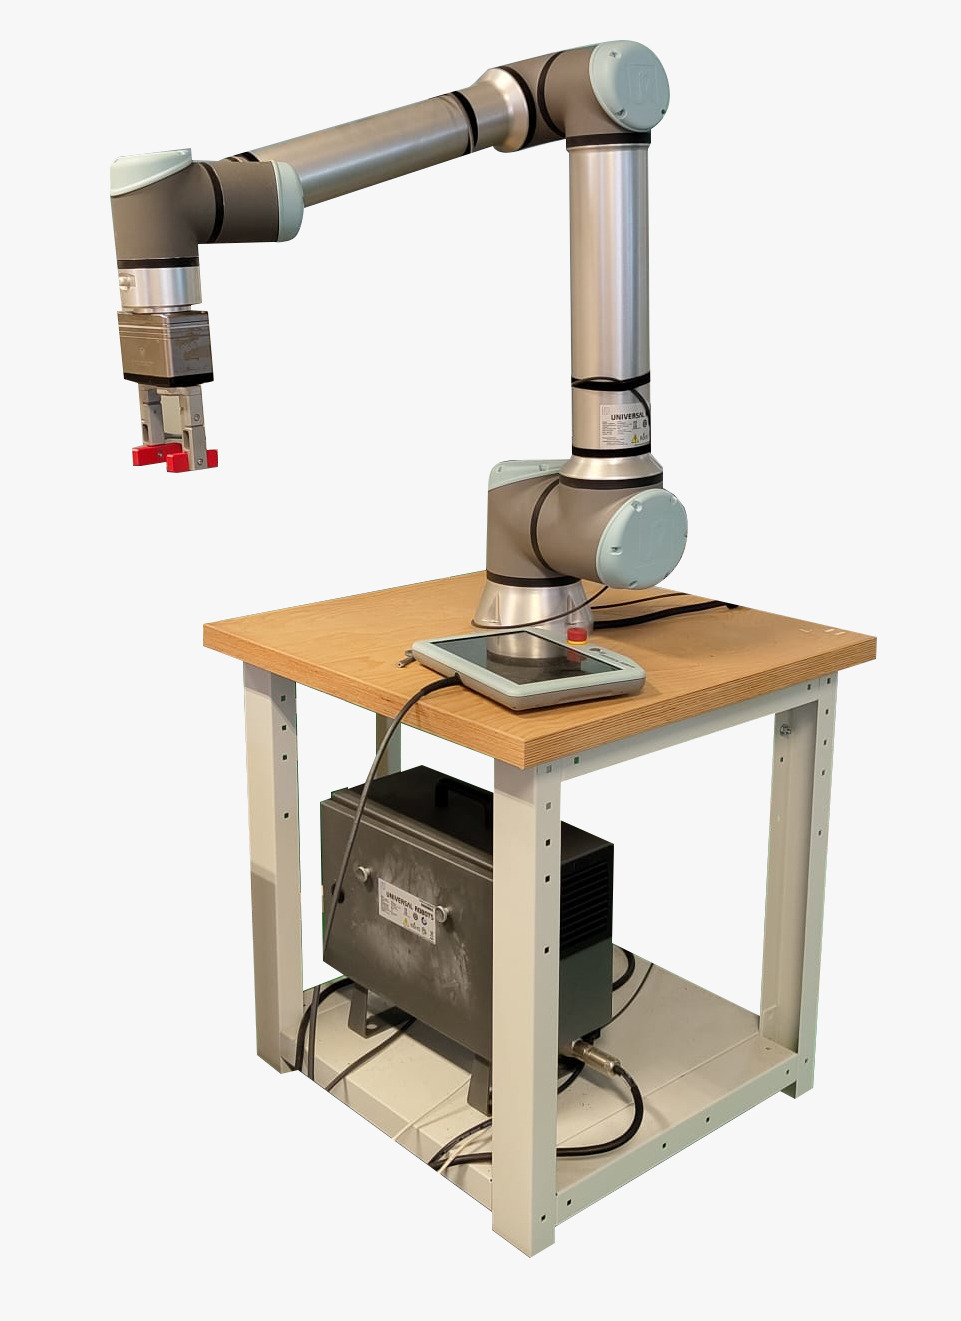
\includegraphics[width=0.4\linewidth]{figs/ur10e.jpeg}
    \caption{Robot UR10e used for the development of the dissertation work, available at IRIS-LAB, University of Aveiro}
    \label{f:ur10e_iris}
\end{figure}

\section{Marker Detection}
\label{section:marker-detection}
% 
% Vuforia is a software platform that enables the creation of \ac{ar} experiences. 
% % Integrated with Unity, a leading platform for developing games and interactive applications, Vuforia simplifies the incorporation 
% of AR into mobile and digital apps. 
% It uses computer vision technologies to recognize and track images and objects in the real world, allowing developers to overlay digital 
% content precisely.

% The marker illustrated in Figure \ref{f:aruco_marker} was selected following initial attempts that yielded inconsistent results when using 
% the laptop's camera, shown in the figure \ref{fig:camera-c922}, to scan the environment. This particular marker demonstrated greater stability, 
% enabling the precise positioning of the digital UR10 model in alignment with the physical surroundings. Consequently, this facilitated the accurate 
% overlay of the digital UR10 model onto the actual UR10e robot, enhancing the integration of virtual and real-world elements.

% \begin{figure}[h]
%     \centering
%       \begin{subfigure}[b]{0.45\textwidth}
%       \centering
%       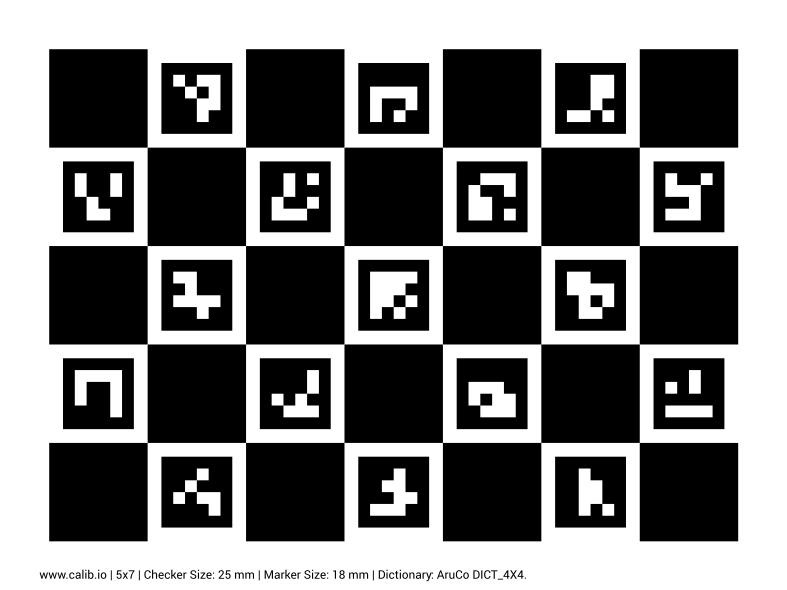
\includegraphics[width=0.7\textwidth]{figs/calib_io_charuco_200x150_5x7_25_18_DICT_4X4.png}
%       \caption{ArUco marker used to allow the segmentation for aligning the digital twin accordingly to the real environment}
%       \label{f:aruco_marker}
%       \end{subfigure}
%         \hfill % This command adds space between the subfigures
%       \begin{subfigure}[b]{0.45\textwidth}
%           \centering
%           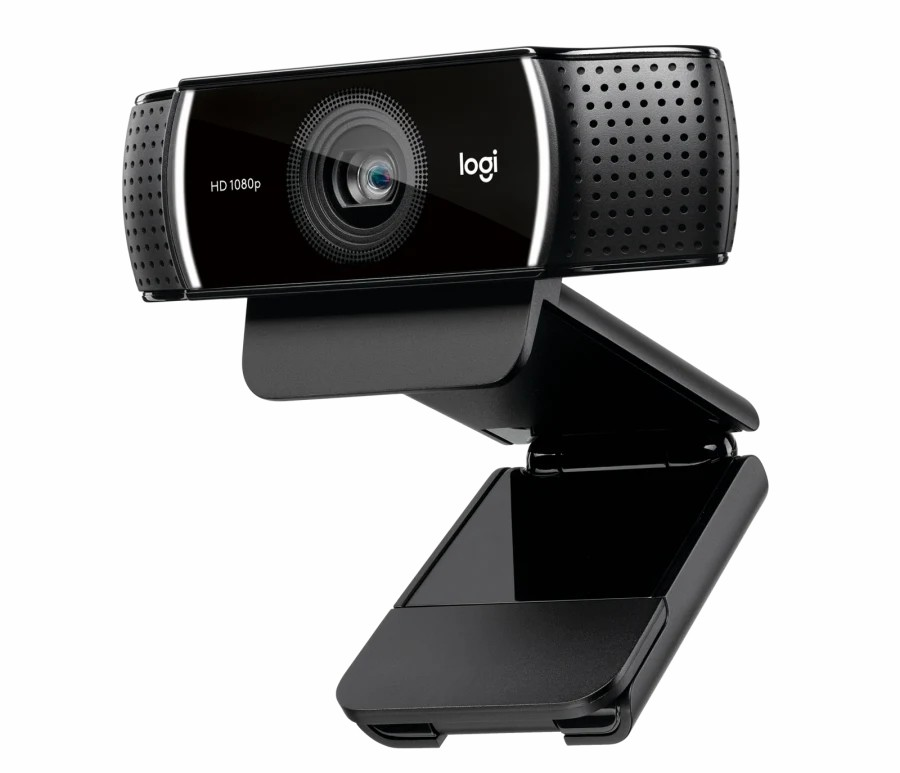
\includegraphics[width=0.7\linewidth]{figs/camera-c922.jpg}
%           \caption{Logitech c922 camera, used for testing on-site application developments}
%           \label{fig:camera-c922}
%       \end{subfigure}
%       \caption{ArUco marker used with the Logitech c922 camera for segmentation and manipulation of virtual environment}
%   \label{marker-camera}
%   \end{figure}
   commented this part because text is below - choose whether to use this or the text below


    Vuforia is a software platform that enables the creation of \ac{AR} experiences. 
    % Integrated with Unity, a leading platform for developing games and interactive applications, Vuforia simplifies the incorporation 
    of AR into mobile and digital apps. 
    It uses computer vision technologies to recognize and track images and objects in the real world, allowing developers to overlay digital 
    content precisely.

    The marker illustrated in Figure \ref{f:aruco_marker} was selected following initial attempts that yielded inconsistent results when using 
    the laptop's camera, shown in the figure \ref{fig:camera-c922}, to scan the environment. This particular marker demonstrated greater stability, 
    enabling the precise positioning of the digital UR10 model in alignment with the physical surroundings. Consequently, this facilitated the accurate 
    overlay of the digital UR10 model onto the actual UR10e robot, enhancing the integration of virtual and real-world elements.

    \begin{figure}[h]
        \centering
        \begin{subfigure}[b]{0.45\textwidth}
        \centering
        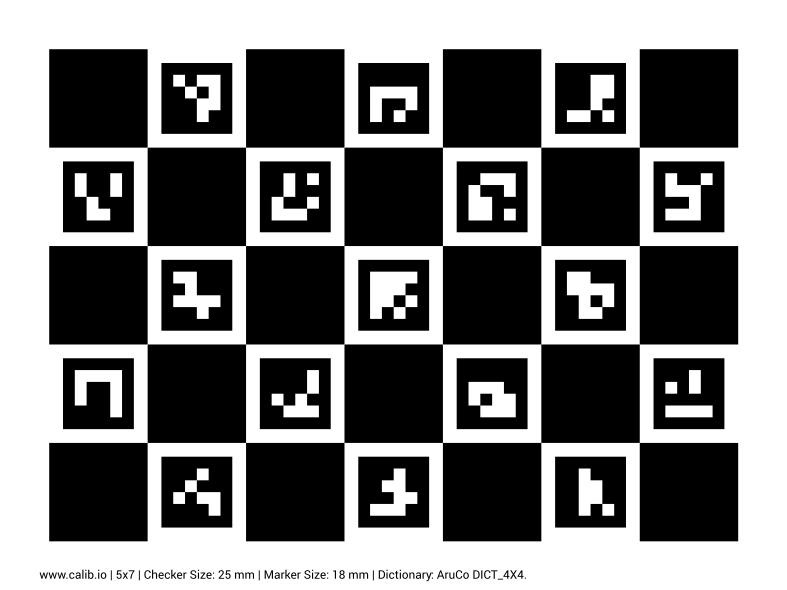
\includegraphics[width=0.7\textwidth]{figs/calib_io_charuco_200x150_5x7_25_18_DICT_4X4.png}
        \caption{ArUco marker used to allow the segmentation for aligning the digital twin accordingly to the real environment}
        \label{f:aruco_marker}
        \end{subfigure}
            \hfill % This command adds space between the subfigures
        \begin{subfigure}[b]{0.45\textwidth}
            \centering
            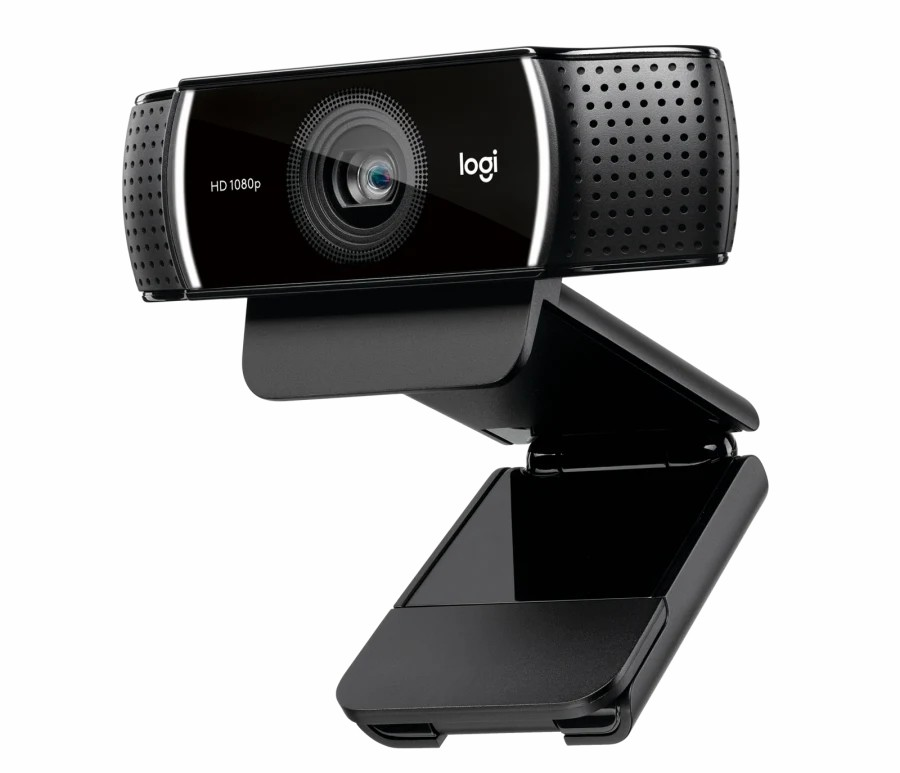
\includegraphics[width=0.7\linewidth]{figs/camera-c922.jpg}
            \caption{Logitech c922 camera, used for testing on-site application developments}
            \label{fig:camera-c922}
        \end{subfigure}
        \caption{ArUco marker used with the Logitech c922 camera for segmentation and manipulation of virtual environment}
    \label{marker-camera}
    \end{figure}
    

\section{Digital Model Implementation of the Robot}
\label{section:digital-model}
% % % foi necessário encontrar um modelo do robot a ser utilizado - UR10e que se encontra no IRIS lab
% To successfully develop the XR application for controlling the UR10e robot, it was essential to identify a model that closely mirrors 
% the actual robot. The Unity Robotics Hub \footnote{Unity Technologies \url{https://github.com/Unity-Technologies/Unity-Robotics-Hub} 
% Accessed: 2024-02-02} facilitates the integration of robotics into Unity projects via the URDF-Importer package 
% \footnote{Unity Technologies \url{https://github.com/Unity-Technologies/URDF-Importer} Accessed: 2024-02-02}. 
% However, challenges arose when attempting to import the UR10e \textit{.urdf} model into the Unity environment. To overcome this, 
% a UR10 model, sourced from a GitHub repository \footnote{PositronicsLab \url{https://github.com/PositronicsLab/reveal_packages/tree/master/industrial_arm/scenario/models/urdf/ur10} Accessed: 2024-02-05} 
% was used, due to its resemblance to the UR10e robot. This was discussed with the educators overseeing the dissertation development, 
% and it was agreed that this approach would not pose any issues.

% In the figure \ref{f:ur10_marker_unity} it is possible to see the digital UR10 model positioned related to the aruco marker 
% (\ref{f:aruco_marker}), in a simulated Unity environment.
% \begin{figure}[h]
% \centering
% 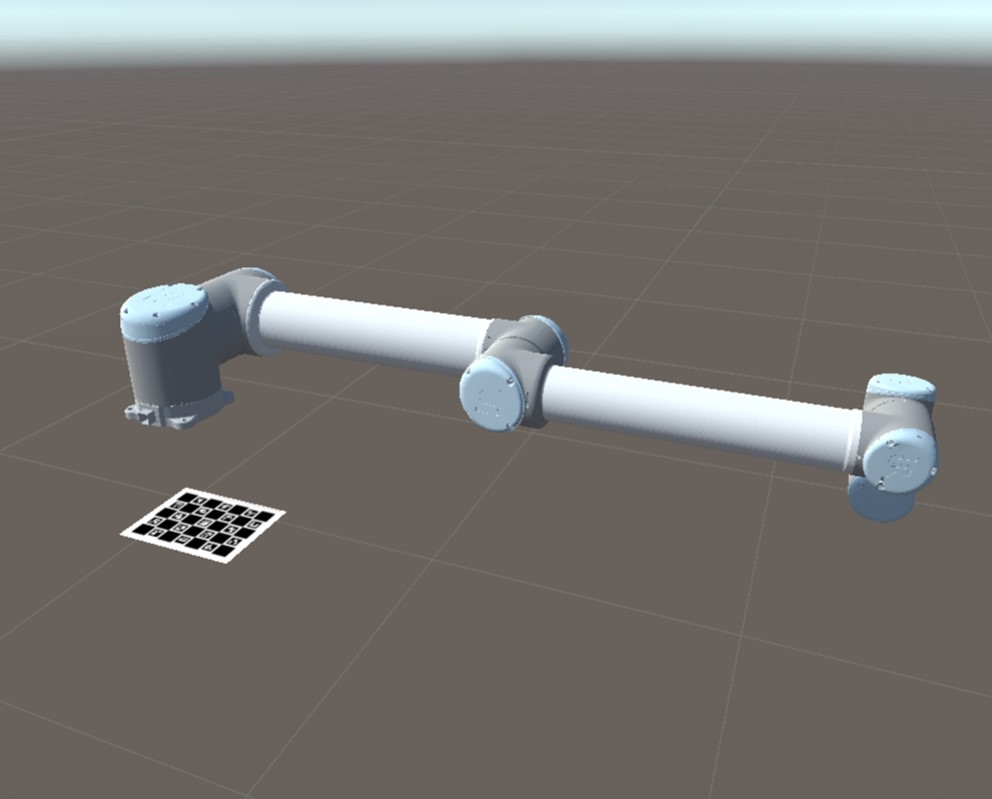
\includegraphics[width=0.6\textwidth]{figs/robot_marker_unity.jpg}
% \caption{Digital UR10 model related to the aruco marker, on Unity environment}
% \label{f:ur10_marker_unity}
% \end{figure}
 - commented this part because text is below - choose whether to use this or the text below

    % foi necessário encontrar um modelo do robot a ser utilizado - UR10e que se encontra no IRIS lab
    To successfully develop the XR application for controlling the UR10e robot, it was essential to identify a model that closely mirrors 
    the actual robot. The Unity Robotics Hub \footnote{Unity Technologies \url{https://github.com/Unity-Technologies/Unity-Robotics-Hub} 
    Accessed: 2024-02-02} facilitates the integration of robotics into Unity projects via the URDF-Importer package 
    \footnote{Unity Technologies \url{https://github.com/Unity-Technologies/URDF-Importer} Accessed: 2024-02-02}. 
    However, challenges arose when attempting to import the UR10e \textit{.urdf} model into the Unity environment. To overcome this, 
    a UR10 model, sourced from a GitHub repository \footnote{PositronicsLab \url{https://github.com/PositronicsLab/reveal_packages/tree/master/industrial_arm/scenario/models/urdf/ur10} Accessed: 2024-02-05} 
    was used, due to its resemblance to the UR10e robot. This was discussed with the educators overseeing the dissertation development, 
    and it was agreed that this approach would not pose any issues.

    In the figure \ref{f:ur10_marker_unity} it is possible to see the digital UR10 model positioned related to the aruco marker 
    (\ref{f:aruco_marker}), in a simulated Unity environment.
    \begin{figure}[h]
    \centering
    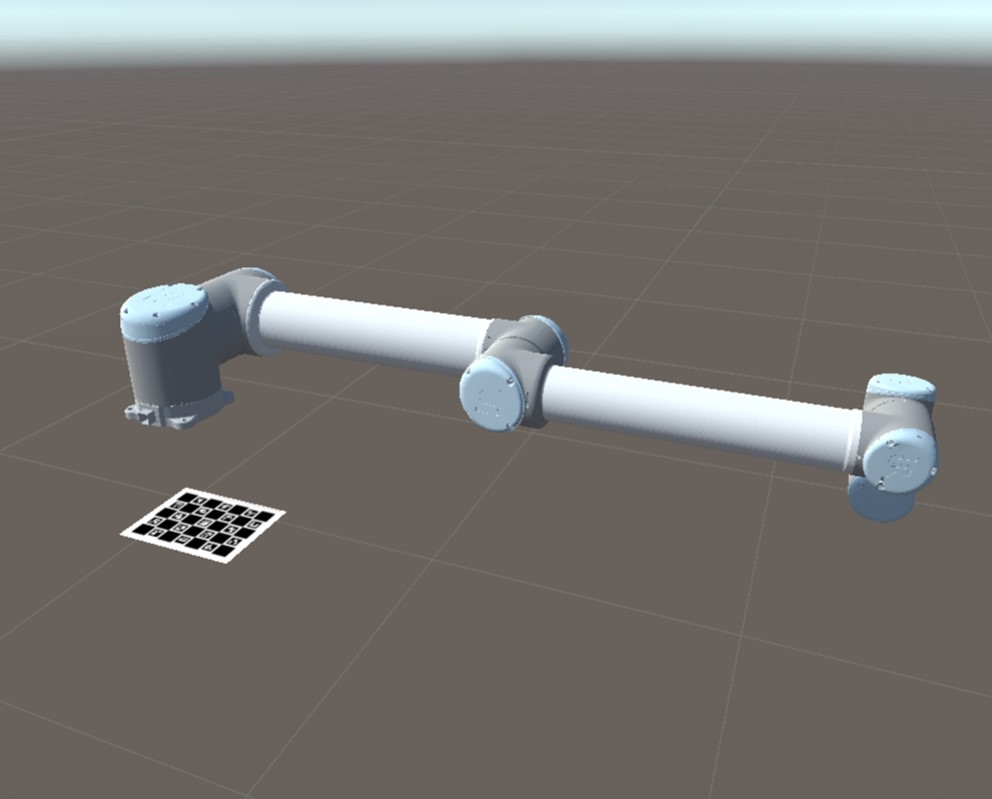
\includegraphics[width=0.6\textwidth]{figs/robot_marker_unity.jpg}
    \caption{Digital UR10 model related to the aruco marker, on Unity environment}
    \label{f:ur10_marker_unity}
    \end{figure}

\section{On-site Application Features}
\label{section:on-site-features}
% \input{chapters/on-site/on-site-features} commented this part because text is below - choose whether to use this or the text below


    The following developed features, for enhancing the on-site environment, work while using a laptop with the camera displayed in 
    the figure \ref{fig:camera-c922}. Despite many attempts, the usage of android handheld devices was not effective, since the digital 
    version of the robot showed physics limitations when entering on the simulation environment.

    \subsection{Virtual Safety Zones}
    \label{subsection:virtual-safety-zones} 
    % \input{chapters/on-site/subsections/virtual-safety-zones} commented this part because text is below - choose whether to use this or the text below


        The implementation of virtual safety zones is a critical feature designed to enhance on-site member's safety when interacting with the robot. 

        Two safety zones were developed, as shown in figure \ref{fig:dual-safety}, to address specific safety and user experience concerns:

        \begin{itemize}
            \item \textbf{Outer Safety Zone}: Initially, only the outer safety zone was developed. The purpose of creating this zone was to provide an 
            early warning to users as they approach the hazardous area near the robot. This approach consisted on changing its color as a visual alert. 
            However, this method proved ineffective because, once inside it, users could not perceive the color change, rendering the warning system inadequate.
            
            \item \textbf{Inner Safety Zone}: To overcome the limitations of the outer zone, an additional, inner safety zone was introduced. 
            This design ensures a two-step safety mechanism:

                \textbf{Visual Alert}: Upon entering the outer safety zone, the color of the inner sphere changes to red. 
                This alteration serves as a visual cue, indicating that the user is getting closer to a high-risk area.

                \textbf{Auditory Warning}: Entering the inner safety zone triggers an auditory alarm. This sound alert signifies that the user has 
                breached into the robot working area, enhancing the effectiveness of the safety mechanism.
        \end{itemize}

        \begin{figure}[h]
            \centering
            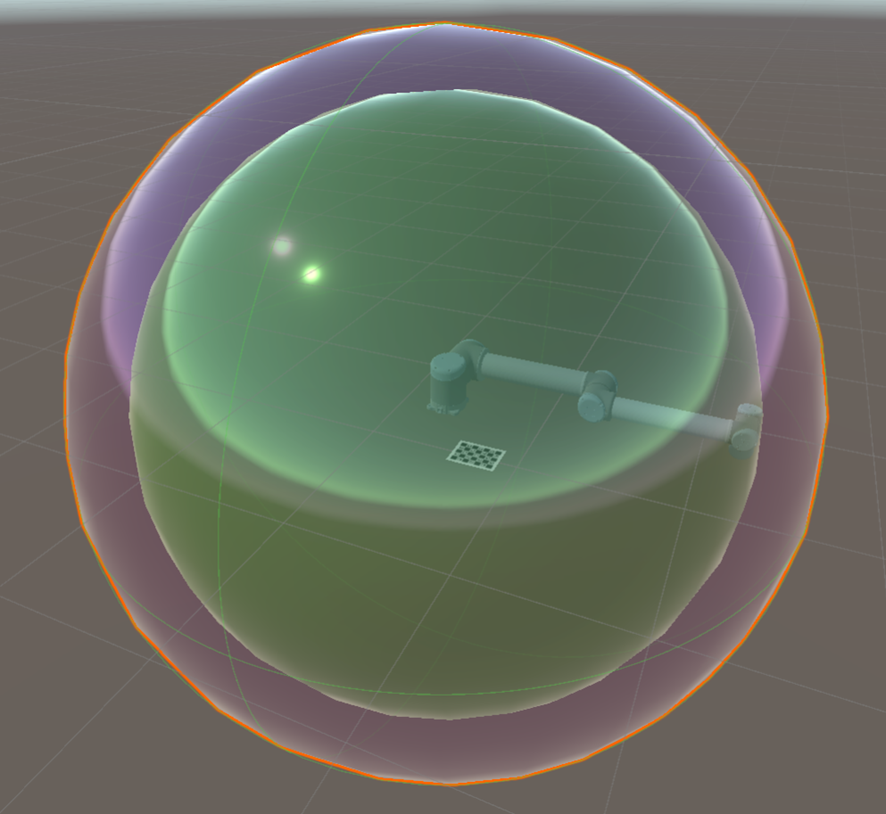
\includegraphics[width=0.5\linewidth]{figs/dual-safetyzone-robot.png}
            \caption{Simulated environment showing the display of both the inner and outer safety zones, as well as the robot and the marker inside them}
            \label{fig:dual-safety}
        \end{figure}

        \subsubsection{Safety Zone Breach Protocol}

            A crucial safety feature is that if the on-site member enters the safety zone area while the robot is in motion, the robot 
            automatically stops. This immediate halt ensures that potential accidents or injuries are avoided by preventing any interaction 
            with the robot when a user is within a designated dangerous area.
                
    \subsection{Interface}

        The interface, which incorporates the safety-zone features detailed earlier, is illustrated in figure \ref{fig: interface}. 
        Within this interface, one can observe the panel for controlling the robot joints'. Additionally, there are two green buttons 
        positioned at the top and bottom right corners of the interface, designated for activating the safety-zone and joint movement functions, 
        respectively. This subsequent features will be explained below.

        \begin{figure}[h]
            \centering
            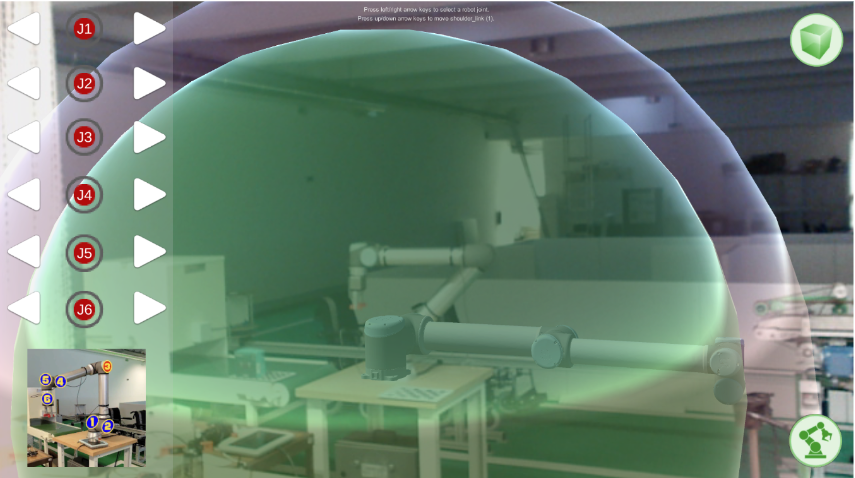
\includegraphics[width=1\linewidth]{figs/interface.png}
            \caption{Interface featuring developed interactions}
            \label{fig: interface}
        \end{figure}

        \subsubsection{Joint Movement}

            This feature allows users to manipulate the robot's joints via a user-friendly interface, as depicted in the figure \ref{fig:joint-1} 
            by the first joint. Its functionality works as follows:


            \begin{itemize}
                \item \textbf{Joint Selection}: Users can activate a joint by clicking on it. Upon activation, the 
                selected joint's central red circle turns green.
                \item \textbf{Movement Control}: By clicking on the selected joint's directional arrows within the interface, it moves in either a 
                positive or negative direction. This functionality mimics the real-time movement control similar to using keyboard arrow keys, ensuring 
                intuitive operation.
                \item \textbf{Continuous Movement}: The selected joint continues to move until we deactivate its button.
                \item \textbf{Single Joint Activation}: To ensure precise control, joint movement is only possible when one joint is selected at a time. 
                This prevents unintended actions and enhances the accuracy of adjustments.
            \end{itemize}
        
        
        \subsubsection{Buttons}
        
            Two buttons, shown in figure \ref{fig:joint-toggle}, were introduced to toggle the activation and deactivation of the joint menu 
            functionalities \ref{fig:toggle-joint} and the safety zones \ref{fig:toggle-safety}. Upon deactivation, the button will turn gray. 
            This design allows users to easily switch these features on or off, providing flexibility in controlling the safety mechanisms and movement 
            operations within the \ac{XR} environment.
            
            
            \begin{figure}[h]
            \centering
            \begin{subfigure}[b]{0.31\textwidth}    
                \centering
                
\includegraphics[width=1\linewidth]{figs/joint-1.png}
                \caption{Joint Control for first Joint}
                \label{fig:joint-1}
                \end{subfigure}
            \hfill % This command adds space between the subfigures
            \begin{subfigure}[b]{0.31\textwidth}
                \centering
                
\includegraphics[width=0.3\linewidth]{figs/clicked_joints.png}
                \caption{Controller Menu Toggle}
                \label{fig:toggle-joint}
            \end{subfigure}
            \hfill
            \begin{subfigure}[b]{0.31\textwidth}
                \centering
                
\includegraphics[width=0.3\linewidth]{figs/unclick_sz.png}
                \caption{Safety-zone Toggle}
                \label{fig:toggle-safety}
            \end{subfigure}
            \caption{Example from first joint control menu and toggle buttons for controller menu and safety-zones}
            \label{fig:joint-toggle}
            \end{figure}
        
\section{Video Demo}
    The video demonstration (\href{https://www.youtube.com/watch?v=SMQ0yXhdnUo}{https://www.youtube.com/watch?v=SMQ0yXhdnUo}) showcases 
    the successful implementation of the previously described features. Testing of the application was conducted using a laptop paired
     with the camera depicted in the figure \ref{fig:camera-c922}. This approach was chosen due to encountered challenges in properly
      building the application for android \ac{HHD}.
            